
\section{Dataset: evaluations and preparations}
\label{sec:InformationsAndAvaliations}

For the development of this work, real field data were used. The data was provided by \cite{equinor2018volve} and is from the Volve field in the Norwegian continental shelf (NCS). This field was discovered in 1993 and it is located in the central part of the North Sea. The production of the field started in 2008. The image above is a crop from the NCS map with contains the Volve field domain, this image was taken from the Norwegian Petroleum \cite{directorate2017factpages}.

\begin{figure}[h!]
    \centering
    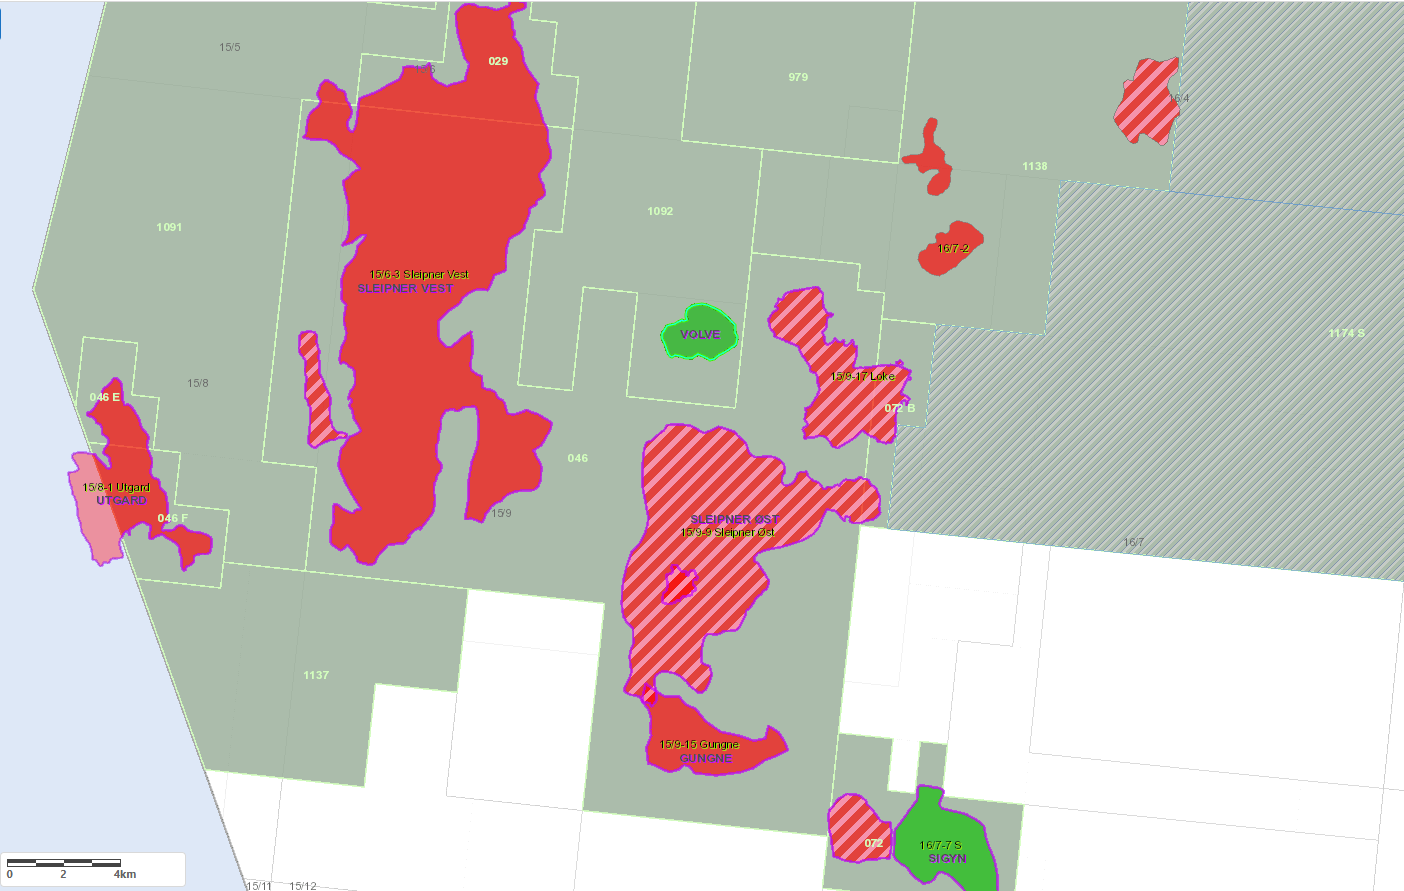
\includegraphics[width=1.0\textwidth]{images/volve_field_my.png}
    \caption{crop from the NCS map that contains the Volve field domain.}
    \label{fig:volve_field}
\end{figure}

In the dataset provided by \cite{equinor2018volve}, there are different types of data such as production data, geological information, reservoir modeling, seismic, and others. This work is focused on the production data, but there are other works such as \cite{sen2019estimation}, and \cite{ravasi2015vector} that contain information about the other available data.

The production dataset contains information that is crucial for planning future activities and understanding the behavior of the field. The file has information about the injections, productions, and observations wells that compose the field. In this work, was used the productor well with the code NO15-9-F-12-H. Figure \ref{fig:all_features} display the different time series that are available in the dataset.

Despite the average from the downhole pressure (\emph{$avg\_downhole\_pressure$}) and the average from the downhole temperature (\emph{$avg\_downhole\_temperature$}) being available data, it is notable in fig \ref{fig:all_features} that from point 1000 onwards both series remain at zero without showing any variation, this behavior is not consistent with the physics present in the production process or during well closure. Therefore, both series were removed from the machine learning model training process.




% \begin{figure}[h!]
%     \centering
%     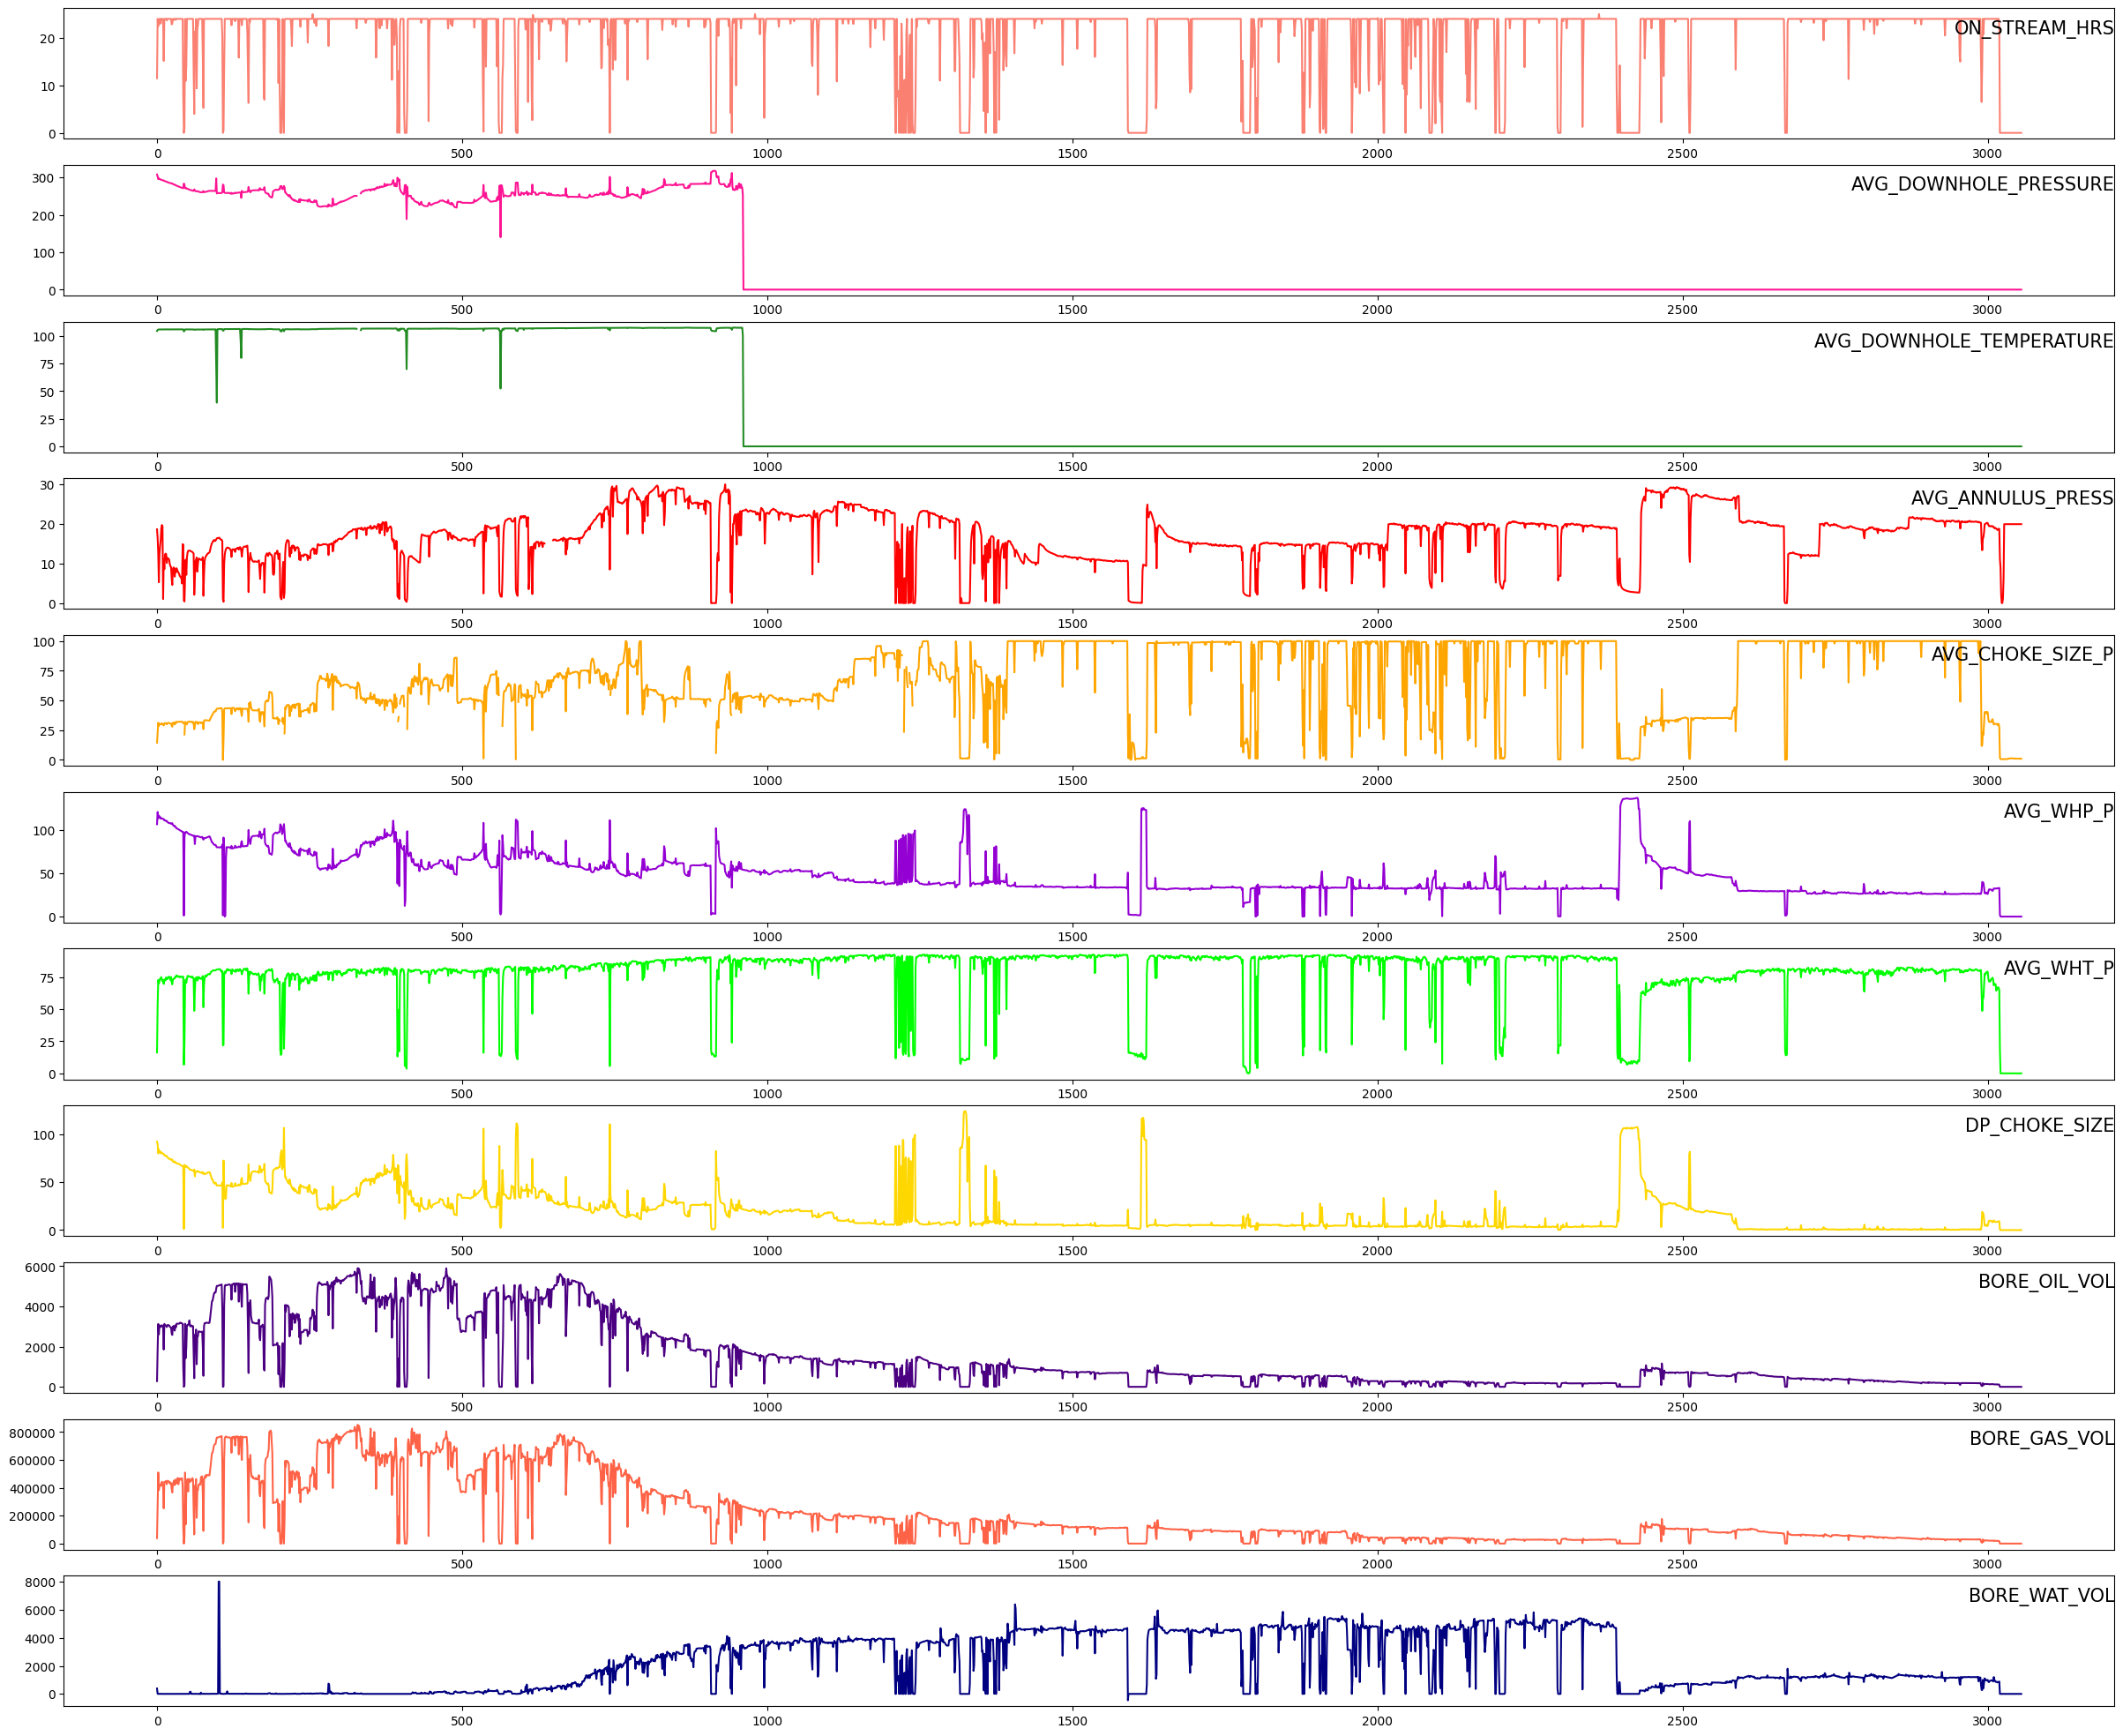
\includegraphics[width=1.0\textwidth]{images/all_features.png}
%     \caption{Time series available to be used in the forecasting process.}
%     \label{fig:all_features}
% \end{figure}

\begin{figure}[h!]
    \centering
    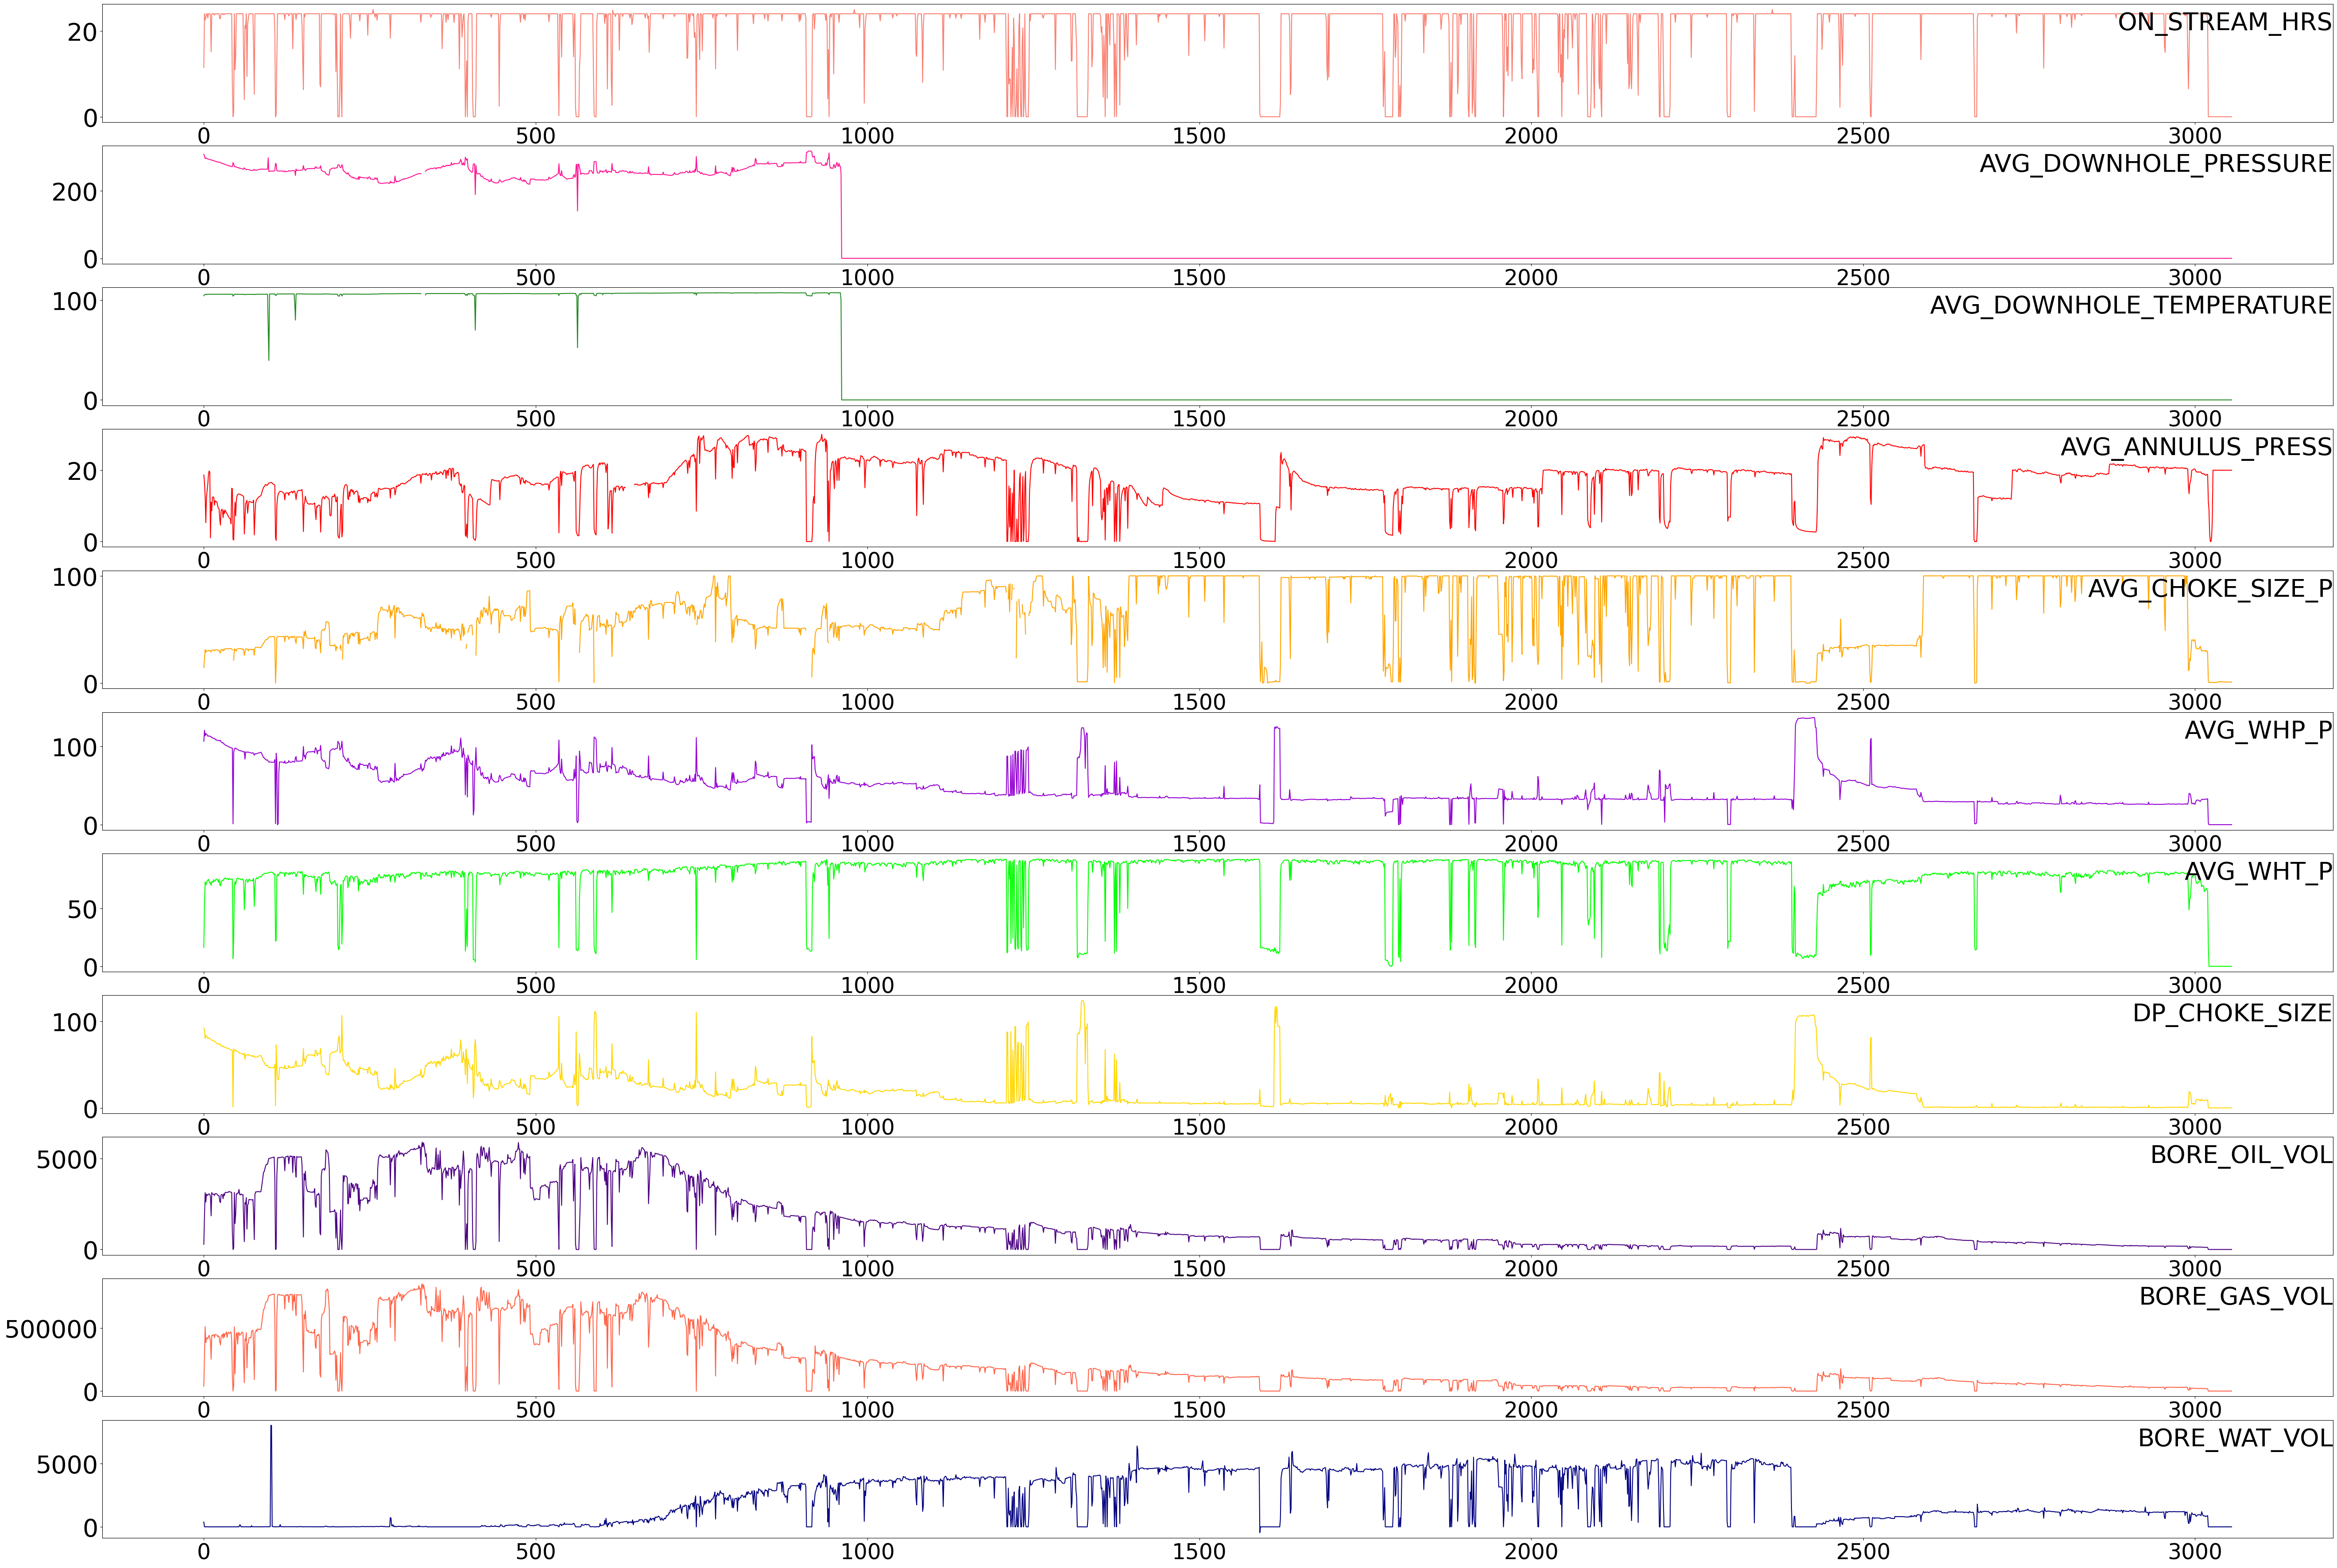
\includegraphics[width=1.0\textwidth]{images/Features3.png}
    \caption{Time series available to be used in the forecasting process.}
    \label{fig:all_features}
\end{figure}


Table with all the variables used in the model.

\begin{center}
\begin{tabular}{ |c|c|c|c| } 
%##############################################
% INFORMACOES PARA PREENCHER A TABELA
% https://discovervolve.com/2020/04/02/__how_to_access_volve/#Production-data_content
%#############################################
\hline
Column name & Type & Definition \\
\hline
% \multirow{3}{4em}{Multiple row} & cell2 & cell3 \\ 
DATEPRD & Data time & Date of production \\ 
ON$\_$STREAM$\_$HRS & Float & Onstream hours  \\ 
AVG$\_$DP$\_$TUBING & Float & Average of pressure differential in tubing \\ 
AVG$\_$CHOKE$\_$SIZE$\_$P & Float & Average of choke size                \\ 
AVG$\_$WHP$\_$P & Float & Average of well head pressure                  \\ 
AVG$\_$WHT$\_$P & Float & Average of well head temperature               \\ 
D$\_$CHOKE$\_$SIZE & Float & Choke size \\ 
BORE$\_$OIL$\_$VOL & Float & Volumetric data for produced oil \\ 
BORE$\_$GAS$\_$VOL & Float & Volumetric data for produced gas \\ 
BORE$\_$WAT$\_$VOL & Float & Volumetric data for produced water \\
\hline
\end{tabular}
\label{tab:Features}
\end{center}

\begin{figure}[h!]
    \centering
    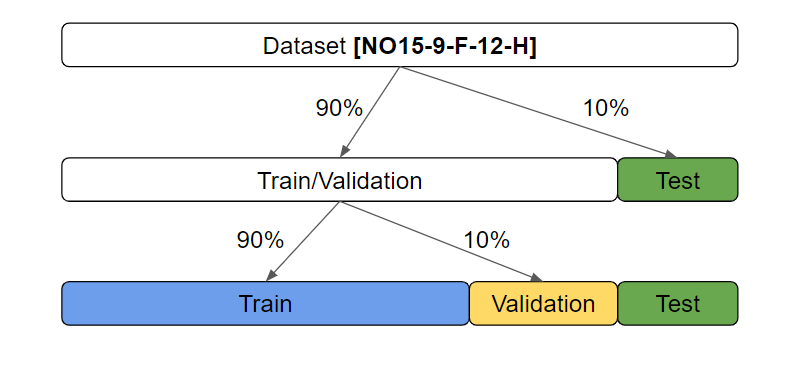
\includegraphics[width=0.6\textwidth]{images/dataset_split.png}
    \caption{Scheme of the split of the dataset in a train, validation, and test subsets.}
    \label{fig:data_split}
\end{figure}